\section{Configuração dos Experimentos}

\subsection{Configurações do Computador}

Esta seção descreve o ambiente de hardware e software utilizado na execução
dos experimentos. O conhecimento dessas configurações é essencial para a
reprodutibilidade dos resultados e para a correta interpretação das métricas
coletadas.

\subsubsection{Hardware}

\paragraph{CPU:}
O processador utilizado é o \textbf{Intel Core i5-13450HX} (13ª geração), com
arquitetura híbrida composta por 6 P-cores (Performance, com Hyper-Threading)
e 4 E-cores (Efficiency, sem Hyper-Threading), totalizando 10 núcleos físicos
e 16 threads lógicas. A frequência máxima é de 4,6 GHz. As memórias cache são:
L1d 416 KiB, L1i 448 KiB, L2 9,5 MiB e L3 20 MiB.

\paragraph{RAM:}
A memória RAM total é de \textbf{16 GB DDR5} em configuração dual-channel
(2 $\times$ 8 GB).

\paragraph{Disco:}
O armazenamento em disco utilizado é um \textbf{SSD NVMe} com capacidade de
512,1 GB.

\subsubsection{Software}

\paragraph{Sistema Operacional:}
\textbf{Ubuntu 24.04.4 LTS}, kernel \texttt{6.17.0-22-generic}.

\paragraph{Java:}
\textbf{OpenJDK 25.0.1} - Temurin-25.0.1+8 (build 25.0.1+8-LTS).

\paragraph{Erlang:}
\textbf{Erlang/OTP 25}, emulador BEAM versão \texttt{13.2.2.5}, com JIT AsmJit habilitado.
    
\subsection{Configurações de Testes}

\subsubsection{Microbenchmark (JMH)}

Os microbenchmarks foram implementados com \textbf{JMH 1.37} sobre \textbf{JDK 25.0.1},
com modo \texttt{AverageTime}, 1 iteração de aquecimento de 10 s, 3 iterações de
medição de 10 s e 1 fork por benchmark. O dataset é carregado uma única vez antes
das medições e uma semente fixa garante reprodutibilidade dos pontos de teste.

\begin{table}[H]
\centering
\begin{tabular}{llp{7cm}}
\hline
\textbf{ID} & \textbf{Método} & \textbf{Objetivo} \\
\hline
B1 & \texttt{b1\_fullRun}         & Execução completa (\textit{k}=10, maxIter=20, tol=\(10^{-6}\)) — número primário do relatório \\
B2 & \texttt{b2\_perIterationCost} & Execução curta (\textit{k}=10, maxIter=5, tol=0) — isola custo por iteração \\
B3 & \texttt{b3\_closestCentroid}  & Chamada isolada de \texttt{closestCentroid} — ponto quente do laço interno \\
B4 & \texttt{b4\_squaredDistance}  & Chamada isolada de \texttt{squaredDistance} — baseline aritmético \\
\hline
\end{tabular}
\caption{Casos de benchmark JMH definidos em \texttt{KMeansBenchmark}.}
\label{tab:jmh-cases}
\end{table}

A Figura~\ref{fig:jmh-config} apresenta a classe de benchmark com as anotações
de configuração e os quatro métodos medidos.

\begin{figure}[H]
    \centering
    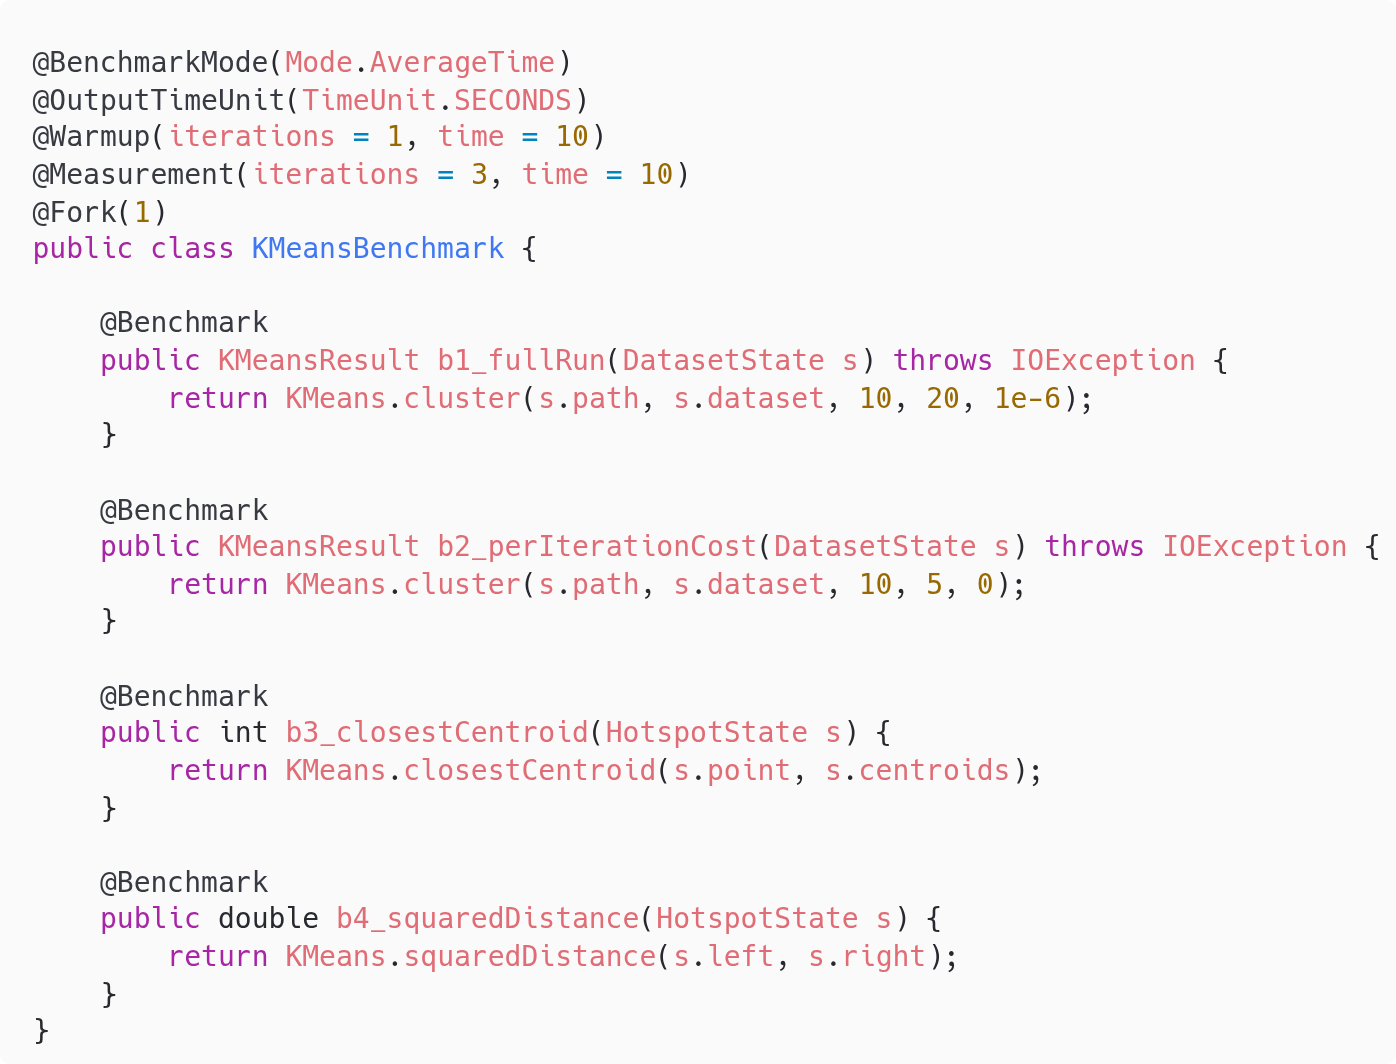
\includegraphics[width=0.85\textwidth]{img/2-configs/jmh-config}
    \caption{Configuração JMH e casos de benchmark em \texttt{KMeansBenchmark}.}
    \label{fig:jmh-config}
\end{figure}

\subsubsection{Macrobenchmark (JMeter)}

Os macrobenchmarks foram implementados com \textbf{Apache JMeter 5.6.3} utilizando
o mecanismo de \textit{Java Sampler} (\texttt{AbstractJavaSamplerClient}). A classe
\texttt{KMeansSampler} executa \texttt{KMeans.cluster()} diretamente na JVM do
JMeter --- sem servidor HTTP intermediário --- permitindo que o coletor de GC
configurado na inicialização do JMeter se aplique integralmente ao algoritmo.

O GC é selecionado pela variável de ambiente \texttt{GC\_ALGO} passada ao script
de inicialização do JMeter. Foram avaliados três coletores:

\begin{itemize}
    \item \texttt{-XX:+UseG1GC} — G1GC (coletor padrão do JDK 25);
    \item \texttt{-XX:+UseZGC} — ZGC (coletor de baixa pausa);
    \item \texttt{-XX:+UseParallelGC} — ParallelGC (coletor paralelo de alta vazão).
\end{itemize}

A matriz de testes combina os três coletores com cinco contagens de threads,
totalizando 15 execuções independentes:

\begin{table}[H]
\centering
\begin{tabular}{ll}
\hline
\textbf{Parâmetro} & \textbf{Valor} \\
\hline
Coletores de GC      & G1GC, ZGC, ParallelGC \\
Threads JMeter       & 1, 2, 4, 8, 16 \\
Duração por execução & 120 s \\
Ramp-up              & 30 s \\
\textit{k}           & 10 \\
maxIter              & 3 \\
tol                  & 0,0 \\
Métrica primária     & Throughput (execuções/min) \\
\hline
\end{tabular}
\caption{Configuração do macrobenchmark JMeter.}
\label{tab:jmeter-config}
\end{table}

\subsubsection{Stress Test (JCStress)}

Os testes de condição de corrida foram implementados com \textbf{JCStress 0.16} e
executados sobre \textbf{JDK 25.0.1}. O JCStress executa múltiplos processos
paralelos variando configurações de compilação e afinidade de CPU, maximizando
a cobertura de possíveis intercalações entre threads.

\begin{table}[H]
\centering
\begin{tabular}{ll}
\hline
\textbf{Parâmetro} & \textbf{Valor} \\
\hline
Ferramenta         & JCStress 0.16 \\
Preset             & \texttt{default} \\
Forks por teste    & 6 (1 normal + 5 stress) \\
Iterações por fork & 5 \\
Tempo por iteração & 1.000 ms \\
CPUs utilizadas    & 16 \\
\hline
\end{tabular}
\caption{Configuração do stress test JCStress.}
\label{tab:jcstress-config}
\end{table}

Foram definidos quatro testes, cada um associado a uma região crítica do algoritmo:

\begin{table}[H]
\centering
\begin{tabular}{llp{6.5cm}}
\hline
\textbf{ID} & \textbf{Classe} & \textbf{Região crítica} \\
\hline
JCS1 & \texttt{JCS1\_ClosestCentroidTest}       & Leitura concorrente do snapshot de centróides \\
JCS2 & \texttt{JCS2\_SquaredDistanceTest}        & Leitura concorrente de \texttt{double[]} compartilhado \\
JCS3 & \texttt{JCS3\_LocalCountAccumulationTest} & \texttt{counts[0]++} em array compartilhado (abordagem ingênua) \\
JCS4 & \texttt{JCS4\_LocalSumAccumulationTest}   & \texttt{sums[0] += 1.0} em array compartilhado (abordagem ingênua) \\
\hline
\end{tabular}
\caption{Testes JCStress e regiões críticas associadas.}
\label{tab:jcstress-tests}
\end{table}

\subsubsection{Profile (JFR)}

O profile foi capturado com \textbf{JFR (Java Flight Recorder)}, ferramenta embutida
no JDK 25 --- sem necessidade de instalação adicional. A gravação foi iniciada via
flag de JVM na execução do algoritmo e analisada exclusivamente com a ferramenta
de linha de comando \texttt{jfr} do JDK, sem uso do JMC (\textit{Java Mission Control}).

A configuração \texttt{settings=profile} habilita amostragem de CPU em alta resolução
(intervalo de 10 ms), adequada para identificar hot methods. A flag
\texttt{dumponexit=true} garante que o arquivo \texttt{.jfr} seja gravado ao final
da execução mesmo sem intervenção manual.

\begin{table}[H]
\centering
\begin{tabular}{ll}
\hline
\textbf{Parâmetro} & \textbf{Valor} \\
\hline
Ferramenta         & JFR (JDK 25 built-in) \\
Configuração       & \texttt{settings=profile} \\
Captura            & \texttt{dumponexit=true} \\
Análise            & \texttt{jfr print} (CLI) \\
GC                 & G1GC \\
\textit{k}         & 10 \\
maxIter            & 3 \\
Dataset            & $\approx$1 GB \\
\hline
\end{tabular}
\caption{Configuração do profile JFR.}
\label{tab:jfr-config}
\end{table}

Os eventos analisados cobrem quatro áreas:

\begin{itemize}
    \item amostras de CPU por método (identificação dos hot methods);
    \item pausas e uso de heap do coletor de GC;
    \item carga de CPU por thread e número de threads ativas;
    \item eventos de leitura de arquivo (bytes lidos, duração).
\end{itemize}

\subsubsection{Microbenchmark em Erlang}

Os microbenchmarks Erlang utilizam \texttt{timer:tc/1}, função nativa do OTP que
mede o tempo de execução de uma fun com resolução de microssegundos. São executadas
1 iteração de aquecimento e 3 de medição, com o dataset carregado uma única vez em
memória antes de qualquer medição para eliminar o custo de I/O dos resultados.
São medidos três casos equivalentes ao JMH: execução completa do algoritmo (B1),
\texttt{closest\_centroid} isolado (B3) e \texttt{squared\_distance} isolado (B4).

\subsubsection{Profile em Erlang}

O profile Erlang coleta métricas de tempo e GC via funções nativas do OTP, sem
necessidade de ferramentas externas. São capturados: tempo de CPU, tempo de parede,
número de coletas GC e utilização média dos schedulers BEAM. O profile cobre uma
execução completa do algoritmo com $k=10$ e \texttt{maxIter}=10.